\documentclass[12pt]{article}
\usepackage{amsmath,amssymb}
\usepackage{graphicx}
\usepackage{multirow}
\usepackage[usenames,dvipsnames]{xcolor}
\usepackage[utf8]{inputenc}
\usepackage[spanish,es-tabla]{babel}

\begin{document}

\title{Parcial III}
\author{Juan Esteban Murcia}
\date{11 de Abril del 2019}
\maketitle


\section{Introducción}
En el estudio de ecuaciones diferenciales ordinarias, surgen problemas (en este caso problemas de valor inicial) a los cuales no se les puede obtener una solución de manera analitica, por esta razón nacen lo que se conoce como los metodos númericos, cuyo objetivo es encontrar un valor $y_{f}$ de la función deseada, y(x) dados las condiciones de la ecuación diferencial, y un punto inicial.\\
Para la realización de este trabajo se usaran los metodos númericos para la solución de una ecuación diferencial de primer orden, es decir de la forma
\begin{equation}
\frac{dy}{dx} = f(x,y)
\label{f}
\end{equation}
Mas en especifico se usaran los metodos de Euler, Euler mejorado y Runge-Kutta.\\\\
Todos los codigos empleados para la realización de este informe se encuentran en el repositorio \textit{https://github.com/JEMN20001/Dif\_Equ}
\section{Metodos}
\subsection{Euler}
El metodo de Euler, así llamado en honor al matemático Leonhard Euler (1707-1783) plantea lo siguiente:\\

Se sabe que $$\frac{dy}{dx} = \lim\limits_{h\to0}\frac{y(x+h)-y(x)}{h}$$
Ahora bien, se puede afirmar que $$\frac{dy}{dx} \approx \frac{y[x+h)]-y(x)}{h}$$ para valores de h cercanos a 0, por lo que reemplazando en (\ref{f}), se llega a la conclusión que
\begin{equation}
 y(x+h) \approx y(x)+h*f(x,y(x))
 \label{euler}
\end{equation}
por lo que dado un punto inicial $(x_{0},y_{0})$ y la ecuación $y' = f(x,y)$ podemos calcular un punto $(x_{f},y(x_{f}))$ de manera aproximada, utilizando (\ref{euler}).
\subsection{Euler mejorado}
El metodo de Euler mejorado, usa el mismo razonamiento que el metodo de Euler, modificando (\ref{euler}) de la siguiente manera
\begin{equation}
y(x+h) \approx y(x)+\frac{h}{2}(f(x,y(x))+f(x+h,y(x)+hf(x,y(x))))
\label{euler_m}
\end{equation}
que simplemente es un promedio del metodo de euler
\subsection{Runge-Kutta}
Finalmente, el metodo de Runge-Kutta es un metodo más sofisticado, el plantea las siguientes acuaciones $$K_{1} = f(x,y(x))$$$$K_{2} = f(x+\frac{h}{2},y(x)+\frac{hK_{1}}{2})$$$$K_3= f(x+\frac{h}{2}, y(x)+\frac{hK_{2}}{2})$$$$K_{4} = f(x+h, y(x)+hK_{3})$$
Y concluye que 
\begin{equation}
y(x+h) \approx y(x)+\frac{h}{6}(K_{1}+2K_{2}+2K_{3}+K_{4})
\label{runge_kutta}
\end{equation}

\section{Comparación}
Para la revisión de estos tres metodos se hizo uso de la ecuación diferencial
\begin{equation}
\frac{dy}{dt} = 1-t+4y~~y(0) = 1
\label{problema1}
\end{equation}, la cual tiene solución analitica $$y(x) = \frac{4t+19e^{4t} -3}{16}$$\\
Con el uso de MATLAB se realizo una comparaciín de esta ecuación con distintos valores de t y h, los valores obtenidos se encuentran en la Tabla \ref{table1}

\begin{table}[h]
	\centering
	\begin{tabular}{|c|c|c|c|c|c|c|c|c|}
		\hline
		&Euler&Euler&Euler m&Euler m&R-K&R-K&R-K&Exacto\\
		\hline
		t & h=0.01 & h=0.001 & h=0.025 & h=0.01 & h=0.2 & h=0.1 & h=0.05 &\\
		\hline
		0&1&1&1&1&1&1&1&1\\
		\hline
		0.1&1.5953&1.6079&1.6079&1.6089&&1.6089&1.6090&1.6090\\
		\hline
		0.2&2.4645&2.5011&2.5021&2.5048&2.5016&2.505&2.5053&2.5053\\
		\hline
		0.3&3.7390&3.8207&3.8228&3.8289&&3.8294&3.8301&3.8301\\
		\hline
		0.4&5.6137&5.7755&5.7797&5.7918&5.7776&5.7928&5.7941&5.7942\\
		\hline
		0.5&8.3767&8.6771&8.6849&8.7075&&8.7093&8.7118&8.7120\\
		\hline
		1&60.0371&64.3826&64.4979&64.8301&64.4416&64.8581&64.8949&64.8978\\
		\hline
		1.5&426.4082&473.5598&474.8340&479.5159&&478.8193&479.2267&479.2592\\
		\hline
		2&3029.3&3484.2&3496.7&3532.9&3490.6&3535.9&3539.9&3540.2\\
		\hline
	\end{tabular}
	\caption{Comparación de los Metodos}
	\label{table1}
\end{table}
\newpage
\section{Puntos}
\subsection{Graficar una Solucion}
A continucación se presenta una grafica de la solucion de la ecuación  (\ref{problema1}) en el intervalo [0,2], generado con el metodo de Euler
\begin{figure}[h]
	\centering
	\caption{}
	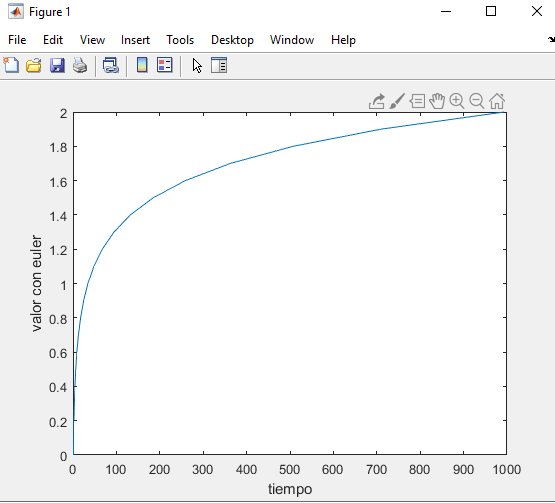
\includegraphics[scale=0.3]{graf1.png}
	\label{graf1}
\end{figure}
\subsection{Comparar Soluciones}
La figura \ref{graf2} representa laa gráficas de la solución de (\ref{problema1}) para distintos h, y la gráfica de la solución analitica
\begin{figure}[h]
	\centering
	\caption{}
	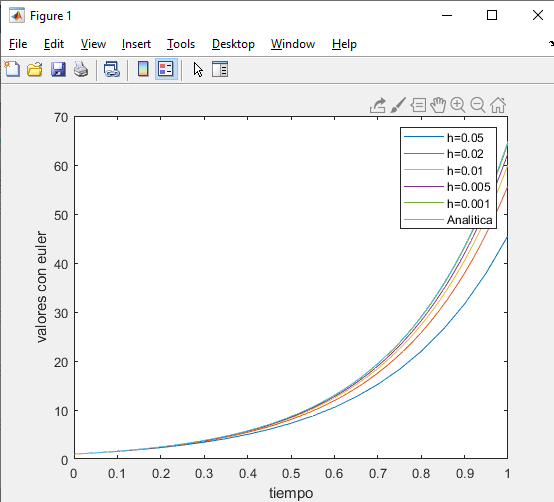
\includegraphics[scale=0.52]{graf2.png}
	\label{graf2}
\end{figure}
\subsection{Calculo de Errores}
Teniendo en cuenta que la ecuación cuenta con una solución analitica, podemos calcular el error como $Err(t) = |y(t)-w(t)|$ donde y es la solución analitica, y w es el valor obtenido con el metodo de euler
\begin{table}[h]
	\centering
	\begin{tabular}{|c|c|c|c|}
		\hline
		t & h=0.1 & h=0.05 & h = 0.01 \\
		\hline
		0.5&2.3878&1.4218&0.3353\\
		\hline
		1&30.4863&19.3094&4.8607\\
		\hline
		1.5&294.3346&197.1873&52.8510\\
		\hline
		2&2546.3&1794.5&510.8722\\
		\hline
	\end{tabular}
\caption{Tabla con los Errores}
\end{table}
\subsection{Euler}
Se tiene la ecuación $$\frac{dy}{dx}+3x^2y=6x^2~~y(0)=3$$
se quiere comprobar que la solución al sistema es
\begin{equation}
y=2+e^{-x^3}
\label{solcuion2}
\end{equation} 
Usando MATLAB, se graficaron las soluciones obtenidas con el metodo de euler para distintos h, y se grafico la funcion (\ref{solcuion2}).
\begin{figure}[h]
	\centering
	\caption{}
	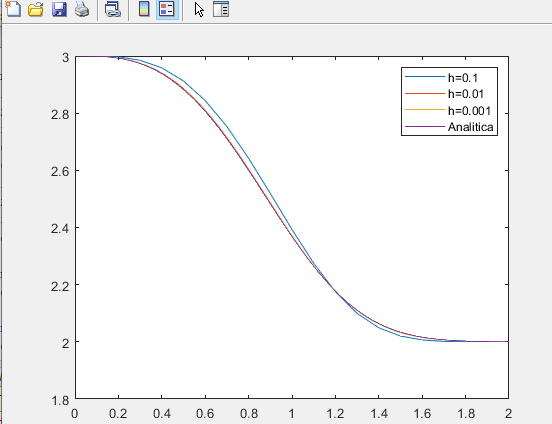
\includegraphics[scale=0.45]{graf3.png}
	\label{graf3}
\end{figure}
\newpage
ademas  se calcularon varios errores presentes en la Tabla \ref{table3}
\begin{table}[h]
	\centering
	\begin{tabular}{|c|c|c|c|}
		\hline
		t & h=0.1 & h=0.001 & h = 0.0001 \\
		\hline
		0.5&0.0299&0.0031&$3.0606x10^{-4}$\\
		\hline
		1&0.0249&0.0022&$2.2097x10^{-4}$\\
		\hline
		1.5&0.0140&0.0012&$1.1856x10^{-4}$\\
		\hline
		2&$3.3593x10^{-4}$&$7.2081x10^{-5}$&$7.6048x10^{-6}$\\
		\hline
	\end{tabular}
	\caption{Tabla con los Errores con Euler}
	\label{table3}
\end{table}
Por lo que podemos conlcuir que la ecuacion(\ref{solcuion2}) es la solución del problema inicial.
\subsection{Runge-Kutta}
Con la misma ecuacción del puto anterior, pero usando el metodo de Runge-Kutta, se obtuvieron los siguientes resultados
\begin{figure}[h]
	\centering
	\caption{}
	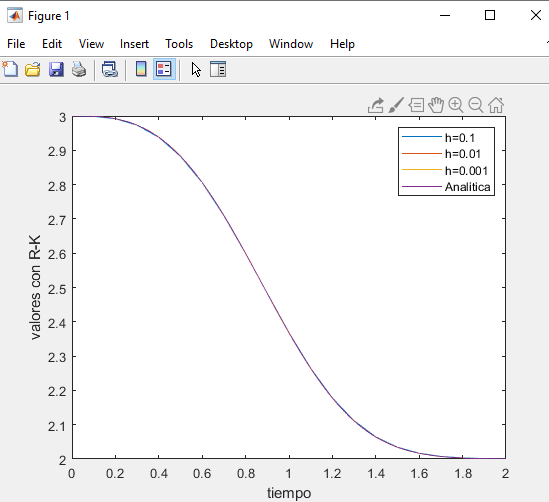
\includegraphics[scale=0.45]{graf4.png}
	\label{graf4}
\end{figure}
\newpage
Tambien se calcularon los errores
\begin{table}[h]
	\centering
	\begin{tabular}{|c|c|c|c|}
		\hline
		t & h=0.1 & h=0.001 & h = 0.0001 \\
		\hline
		0.5&$1.5800x10^{-7}$&$8.6153x10^{-13}$&$8.8818x10^{-16}$\\
		\hline
		1&$6.0669x10^{-6}$&$6.7516x10^{-10}$&$6.4837x10^{-14}$\\
		\hline
		1.5&$8.2371x10^{-5}$&$5.6887x10^{-9}$&$5.4978x10^{-13}$\\
		\hline
		2&$3.0019x10^{-5}$&$1.3747x10^{-9}$&$1.2790x10^{-13}$\\
		\hline
	\end{tabular}
	\caption{Tabla con los Errores con R-K}
	\label{table4}
\end{table}
\subsection{Ven Der Pol}
Dada la ecuación
\begin{equation}
	u''-\mu(1-u^2)u'+u=0,~~u(0)=1, u'(0)=0
	\label{Pol}
\end{equation}
Se puede hacer un cambio de variables $$x = u$$$$y = u'$$
para llegar a un sistema de ecuaciones de primer orden de la forma $$(x',y') = (y, -x+\mu(1-x^2)y),~~(x0,y0)=(1,0)$$ y adaptando el metodo de Runge-Kutta, podemos calcular el valor aproximado en un momento t.

Tomando $\mu = 0.2$ y con 3 valores distontos para h se obtuvieron las gráficas
\begin{figure}[h]
	\centering
	\caption{}
	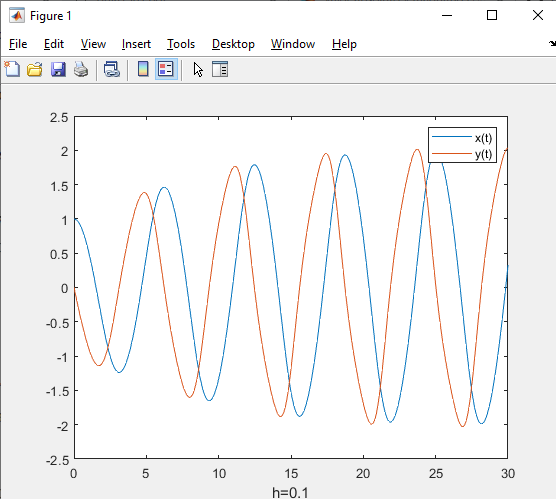
\includegraphics[scale=0.45]{graf5.png}
	\label{graf5}
\end{figure}
\begin{figure}[h]
	\centering
	\caption{}
	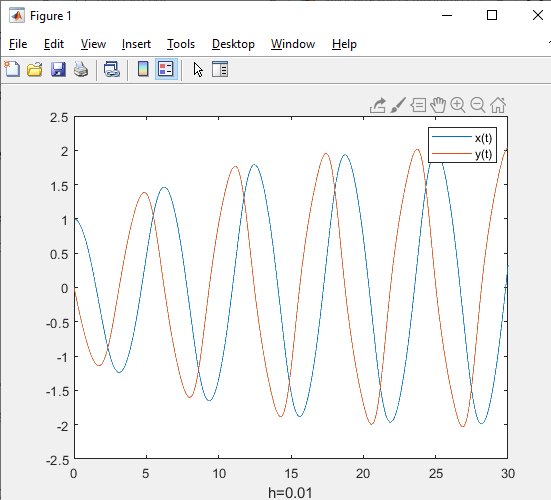
\includegraphics[scale=0.45]{graf6.png}
	\label{graf6}
\end{figure}
Variando las condiciones iniciales a (a,b) (en este caso (-1,-2)) se puede observar que la gráfica de x(t) se desplaza a unidades en la dirección correspondiente, y y(t) se desplaza b unidades en la direccion correspondiente (la cual está dada por el signo de a y de b), esto se puede observar en la figura (\ref{fig8})
\begin{figure}[h]
	\centering
	\caption{}
	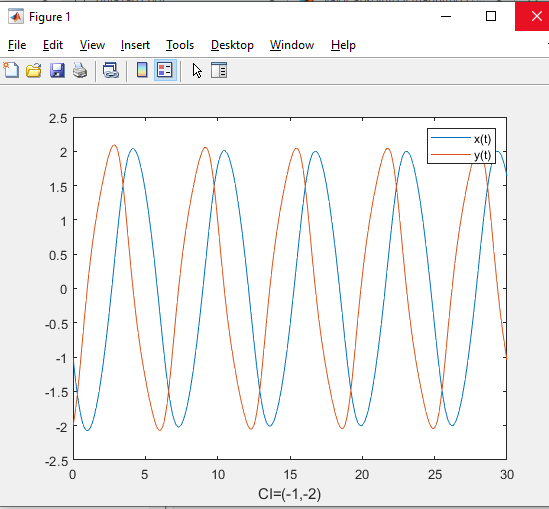
\includegraphics[scale=0.45]{graf8.png}
	\label{graf8}
\end{figure}
\newpage
Y finalmente si se gráfica y(t) con respecto a x(t) se obtiene la gráfica de la figura \ref{graf9}
\begin{figure}[h]
\centering
\caption{}
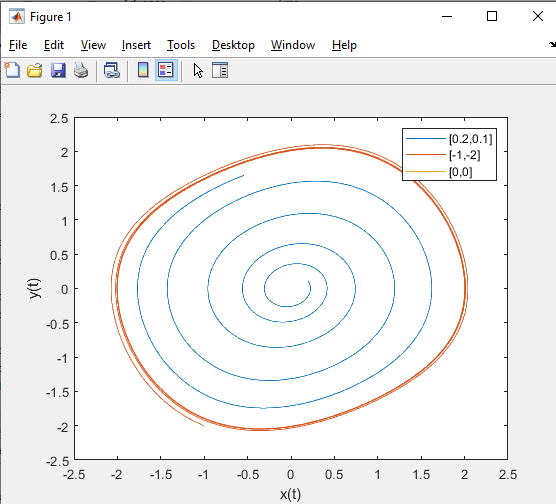
\includegraphics[scale=0.45]{graf9.png}
\label{graf9}
\end{figure}
Finalmente modificando los valores de $\mu$ podemos observar que la gráfica de y con respecto a x se estrecha o se agranda, adicionandole a medida que $\mu$ crece se forma una nueva forma alrededor del origen, este es el gráfico para $\mu = 2$ 
\begin{figure}[h]
	\centering
	\caption{}
	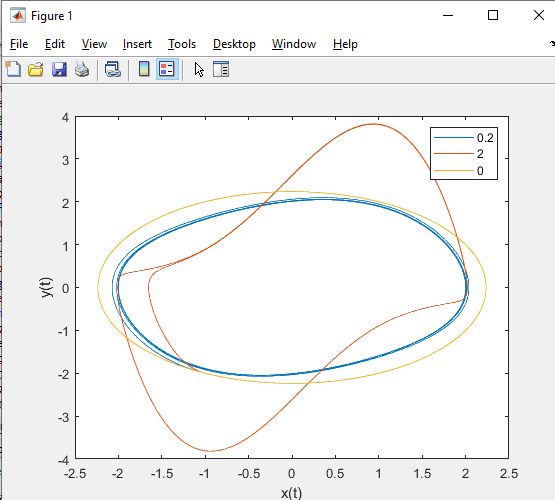
\includegraphics[scale=0.45]{graf10.png}
	\label{graf10}
\end{figure}
\section{Conclusiones}
Con respecto a los 3 metodos presentados en este informe, es evidente que el metodo de Runge-Kutta es el que más se acerca a la solución real, esto se puede observar en las distintas tablas de errores presentadas en este informe.\\\\
Con respecto al problema de Van Der Pol hay mucho que analizar, por ejemplo la importancia del parametro $\mu$ el cual determina el ciclo que va a seguir la gráfica y(t) con respecto a x(t). El valor incial, el cual determina el punto en el que se inicia el ciclo, y esto es importante para poder modelar bien el sistema que se va a estudiar.
\end{document}
